\begin{enumerate}
	\item задание. \\
	
\includegraphics[width=17cm]{1.pdf}
	\inputminted{C}{1.c}
	\newpage

	\item задание. \\
	\includegraphics[width=17cm]{2.pdf}
	\inputminted{C}{2.c}
	\newpage

	\item задание. \\
	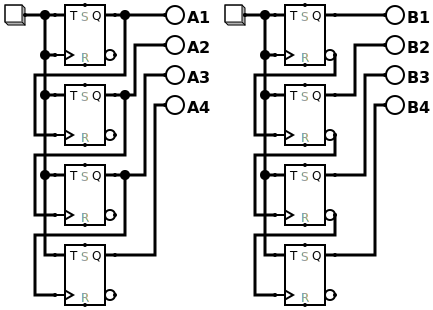
\includegraphics[width=17cm]{3.pdf}
	\newpage
	\inputminted{C}{3.c}
	\newpage

	\item задание. \\
	\includegraphics[width=17cm]{4.pdf}
	\newpage
	\inputminted{C}{4.c}
	\newpage

	\item задание. \\
	
\includegraphics[width=17cm]{5.pdf}
	\newpage
	\inputminted{C}{5.c}
	\newpage

	\item задание. \\
	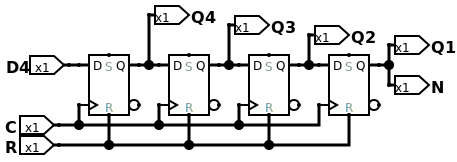
\includegraphics[width=17cm]{6.pdf}
	\newpage
	\inputminted{C}{6.c}
	\newpage

	\item задание. \\
	\includegraphics[width=17cm]{7.pdf}
	\newpage
	\inputminted{C}{7.c}
	\newpage

	\item задание. \\
	\includegraphics[width=17cm]{8.pdf}
	\newpage
	Код на Си (с двойной точностью):
	\inputminted{C}{81.c}
	Вывод: \\
	-1180591620717411303424.000000 \\
	1.172604 \\
	0.000000, 0.000000, 0.000000, 0.000000 \\
	\newpage
	Код на Паскале (с одинарной точностью):
	\inputminted{Pascal}{82.pas}
	Вывод: \\
	576460752300000000.000000 \\
	1.172604 \\
	0.000000, 0.000000, 0.000000, 0.000000 \\
	\newpage
	Код на Питоне:
	\inputminted{Python}{83.py}
	Вывод: \\
	1.1805916207174113e+21 \\
	-0.8273960599468213 \\
	0.0, 0.0, 0.0, 0.0 \\
	\newpage
\end{enumerate}